\documentclass[12pt,a4paper]{article}

\usepackage{geometry}
\geometry{
    left=2cm, 
    right=2cm,
    top=3cm,  
    bottom=2cm
}

\usepackage[english,spanish]{babel}
\usepackage[utf8]{inputenc}
\usepackage{amsmath}

\usepackage{graphicx}
\usepackage{wrapfig}
\usepackage{makecell}
\usepackage{booktabs}

\usepackage{setspace}
\setstretch{1.5}
\setlength{\parindent}{0pt}

\usepackage{csquotes}
\usepackage{hyperref}
\usepackage[style=ieee]{biblatex}
\addbibresource{Referencias.bib}

\begin{document}
    \begin{titlepage}
        \begin{minipage}[c]{0.1\textwidth}
            
\includegraphics[width=\textwidth]{./Resources/logo_unam.jpg}
        \end{minipage}
        \begin{minipage}{0.8\textwidth}
            \centering
            {\Large\textbf{Universidad Nacional Autónoma de México}\\}
            {\large\textbf{Escuela Nacional de Estudios Superiores\\\underline{Unidad Morelia}}}
        \end{minipage}
        \begin{minipage}[c]{0.1\textwidth}
            
\includegraphics[width=\textwidth]{./Resources/logo_enes.jpg}
        \end{minipage}
        \vspace{3cm}

        \centering

        {\large{Proyecto Final\\}}
        {\Large\textbf{Predicción del Crecimiento Significativo en Plantas}}
        \vspace{2cm}

        {{PRESENTA:\\}}
        {\large\textbf{Alexis Uriel Aguilar Uribe}}
        \vspace{1cm} 

        {{PROFESORES:\\}}
        {\large\textbf{Dra.\ Marisol Flores Garrido}}\\
        {\large\textbf{Dr.\ Luis Miguel García Velázquez}}
        \vspace{2cm}

        {{GRADO\\}}
        {\large\textbf{Licenciatura en Tecnologías para la Información en Ciencias}}
        \vspace{2cm}

        \flushleft{
        {\textbf{Número de Cuenta:\ }424060075}\\
        {\textbf{Asignatura:\ }Sistemas basados en conocimiento [Machine Learning]}}
        \vspace{2cm}

        \flushright{
        {\textbf{A:\ }\underline{27 de Mayo del 2025}}}
        \vfill

    \end{titlepage}

    \tableofcontents
    \newpage

    \section{Introducción}
    {
        En la agricultura, como cualquier otra industria, se vuelve relevante la 
        optimización de los recursos y ganancias, es decir, reducir los insumos 
        consumidos mientras se incrementa la producción (tanto en calidad como en 
        cantidad); todo lo anterior se traduce en aplicar mejoras en diferentes 
        áreas y aspectos que convergen y se relacionan para generar ganancias y 
        reducir costos en la agricultura. Para el caso de este proyecto, el interés 
        se encuentra en el crecimiento de las plantas, bajo qué factores ambientales 
        y de cuidado propician un crecimiento significativo en las plantas.\\ 

        Para lograr el último punto, se tiene como objetivo el crear un modelo de 
        aprendizaje supervisado para la clasificación del crecimiento significativo 
        en base a los factores y mediciones relacionadas a su cuidado y ambiente. 
        Esto se encuentra desarrollado en el repositorio en GitHub dedicado para 
        el proyecto: \href{https://github.com/alexisuaguilaru/Plant_Growth_Model}{Plant Growth Model}.\\
    }
    \newpage

    \section{Descripción de los Datos}
    {
        El conjunto de datos que se emplearán para el proyecto se encuentra disponibles 
        en \cite{dataset_plants}, que es un conjunto de datos publicados en \href{https://www.kaggle.com/}{Kaggle} por 
        la propia comunidad. Se cuenta con siete columnas, donde seis de ellas son 
        atributos y la otra el target, referenciando a la fuente del conjunto de datos, 
        se tienen los siguientes atributos junto con su descripción y tipo de dato: 

        \begin{itemize}
            \item \textbf{Soil\_Type       } [\emph{String}]: El tipo o composición del suelo 
            en el que las plantas están creciendo o se plantan.
            
            \item \textbf{Sunlight\_Hours  } [\emph{Float}]: La duración o intensidad de la luz 
            solar que las plantas reciben.
            
            \item \textbf{Water\_Frequency } [\emph{String}]: Qué tan seguido se riegan las 
            plantas, se indica la frecuencia del riego.
            
            \item \textbf{Fertilizer\_Type } [\emph{String}]: El tipo de fertilizante usado 
            para nutrir a las plantas.
            
            \item \textbf{Temperature      } [\emph{Float}]: Las condiciones de la temperatura 
            ambiental bajo las cuales las plantas están creciendo.

            \item \textbf{Humidity         } [\emph{Float}]: El nivel de humedad en el ambiente 
            alrededor de las plantas.

            \item \textbf{Growth\_Milestone} [\emph{Integer, Target}]: Descripción o marcadores 
            que indican la etapa o eventos significativos en el proceso de crecimiento de 
            las plantas.
        \end{itemize}

        Por último, el conjunto de datos consta de $193$ instancias (filas), las diferentes 
        instancias lucen de la siguiente manera:

        \begin{center}    
            \begin{tabular}{lrll}
                \toprule
                Soil\_Type & Sunlight\_Hours & Water\_Frequency & Fertilizer\_Type \\
                \midrule
                sandy & 9.228 & daily     & none     \\
                sandy & 9.774 & weekly    & chemical \\
                clay  & 7.392 & bi-weekly & none     \\
                clay  & 6.462 & bi-weekly & organic  \\
                clay  & 8.846 & weekly    & organic  \\
                loam  & 5.985 & bi-weekly & chemical \\
                \bottomrule
            \end{tabular}
            \begin{tabular}{rrr}
                \toprule
                Temperature & Humidity & Growth\_Milestone \\
                \midrule
                33.804 & 32.815 & 0 \\
                32.549 & 61.377 & 1 \\
                31.100 & 68.600 & 0 \\
                27.517 & 34.175 & 1 \\
                27.700 & 56.800 & 1 \\
                29.757 & 57.476 & 0 \\
                \bottomrule
            \end{tabular}
        \end{center}

    }
    \newpage

    \section{Análisis Exploratorio de Datos}\label{sec:eda}
    {
        Los tipos de datos en base a la descripción proporcionada en \cite{dataset_plants} 
        con la mostrada al momento de la lectura de los datos en Python, por lo que no 
        es necesario realizar una transformación sobre los tipos de datos de cada atributo. \\
        
        Debido a que los valores que toma y representan el target, \emph{Growth\_Milestone}, 
        son enteros, se tiene que el modelo que se generará será un clasificador binario; cuyas clases 
        representan si hay un crecimiento significativo, bajo ciertos criterios, en las plantas. 
        Como primera observación se tiene que el conjunto de datos está balanceado respecto 
        a las clases, por lo que se podría usar cualquiera de las métricas bajo una 
        justificación válida o apropiada al problema:

        \begin{center}
            \begin{tabular}{lr}
            \toprule
                Growth\_Milestone &  \\
                Clases & Conteo \\
            \midrule
                0 [No Milestone] & 97 \\
                1 [Milestone] & 96 \\
            \bottomrule
            \end{tabular}
        \end{center}
        
        Se presenta un análisis univariado sobre los atributos numéricos y categóricos, y 
        por último se prueban algunas hipótesis relevantes y relacionadas sobre las observaciones 
        en los apartados anteriores.

        \subsection{Atributos Numéricos}
        {
            Generando la descriptiva básica (medidas centrales y de dispersión) de 
            los datos se obtienen los siguientes resultados:

            \begin{center}
                \begin{tabular}{lrrr}
                \toprule
                    Medida & Sunlight\_Hours & Temperature & Humidity \\
                \midrule
                    Media               & 6.8264 & 25.0760 & 58.0989 \\
                    Desviación Estándar & 1.5995 &  5.3541 & 12.6317 \\
                    Mínimo              & 4.0331 & 15.2000 & 30.5676 \\
                    $Q_1$               & 5.4770 & 20.6370 & 49.3000 \\
                    $Q_2$               & 6.8332 & 25.9123 & 59.1828 \\
                    $Q_3$               & 8.2411 & 29.7579 & 69.1000 \\
                    Máximo              & 9.9139 & 34.8101 & 79.6482 \\
                \bottomrule
                \end{tabular}
            \end{center}

            Primero se destaca que siguen diferentes rangos de valores, por lo que se 
            tendrán que estandarizar o blanquear para su adecuado uso para el entrenamiento 
            de los modelos que se crearán, además de permitir realizar comparativas entre 
            las distribuciones. Al estandarizar los valores se tienen los siguientes resultados:

            \begin{center}
                \begin{tabular}{lrrr}
                \toprule
                Medida & Sunlight\_Hours & Temperature & Humidity \\
                \midrule
                Media               & 0 & 0 & 0 \\
                Desviación Estándar & 1 & 1 & 1 \\
                Mínimo              & -1.746 & -1.8445 & -2.1795 \\
                $Q_1$               & -0.843 & -0.8290 & -0.6965 \\
                $Q_2$               &  0.004 &  0.1561 &  0.0858 \\
                $Q_3$               &  0.884 &  0.8744 &  0.8709 \\
                Máximo              &  1.930 &  1.8180 &  1.7059 \\
                \bottomrule
                \end{tabular}
            \end{center}

            Destacándose que el atributo \emph{Sunlight\_Hours} figura que sigue una 
            distribución debido a que su $Q_2$ se aproxima a $0$ junto que sus $Q_1$ 
            y $Q_3$ se parecen, salvo el signo. Mientras que en \emph{Humidity} su $Q_2$ 
            se encuentra equidistante a $Q_1$ y a $Q_3$, lo que significa que no tiene 
            sesgo más no es simétrica. Y en \emph{Temperature}, por sus cuartiles, tiene 
            un sesgo negativo considerable. En base a lo mencionado se tiene que los tres 
            atributos siguen diferentes distribuciones, implicando que estos atributos surgen 
            de diferentes fenómenos, interacciones y procesos que impactan en el crecimiento 
            de las plantas, por lo que los tres atributos se vuelven relevantes para la 
            clasificación debido a que cada uno condensa diferentes procesos para lograr un 
            crecimiento significativo.\\

            De los box plots, se puede observar que las distribuciones de los atributos 
            no son tan diferentes según el target, según si hay un crecimiento significativo, 
            esto al ver que las cajas están superpuestas, haciendo que no exista una diferencia 
            Significativa entre las medias de las distribuciones. Lo que se destaca es que 
            cuando existe un crecimiento significativo tiende a tomar valores más bajos y además 
            de que su desviación estándar también tiende a decrecer.\\ 

            Este último hecho se podría relacionar con que existe un control sobre los factores 
            ambientales, haciendo que las distribuciones sean más restrictivas y reguladas, 
            dejando afuera posibles fenómenos que generen un ambiente irregular para el 
            crecimiento de las propias plantas. Haciendo que la planta esté en un ambiente ideal 
            para su crecimiento pero, por las distribuciones, existe la posibilidad de que aunque 
            esté en las condiciones idóneas no logre un crecimiento significativo.

            \begin{figure}[hbtp]
                \centering
                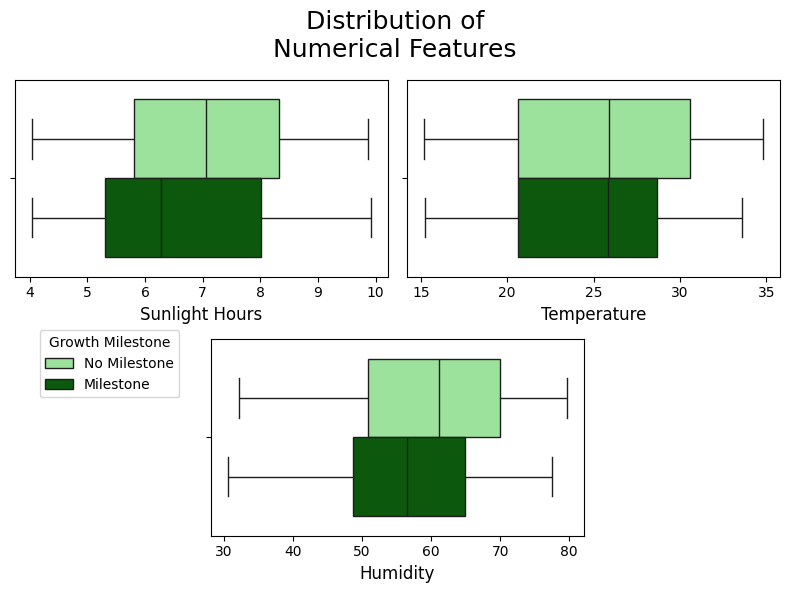
\includegraphics[width=0.95\textwidth]{./Resources/3_1.png}
                \caption{Distribución de los atributos Numéricos según el Crecimiento Significativo}
                \label{fig:dist_num}
            \end{figure}

            De manera visual, no se cuenta con valores atípicos derivados de la Regla del 
            Rango Intercuartil ni valores faltantes, por lo que estos atributos numéricos se 
            encuentran preparados para la fase de entrenamiento.
        }

        \subsection{Atributos Categóricos}
        {
            Cada atributo categórico tiene tres valores únicos, con las siguientes cantidades 
            y valores:\\
                
            \begin{minipage}{0.5\textwidth}
                \centering
                \begin{tabular}{lr}
                    \toprule
                        {Soil\_Type} & {Cantidad} \\
                    \midrule
                        clay & 67 \\
                        sandy & 64 \\
                        loam & 62 \\
                    \bottomrule
                \end{tabular}
            \end{minipage}%
            \begin{minipage}{0.5\textwidth}
                \centering
                \begin{tabular}{lr}
                    \toprule
                        {Water\_Frequency} & {Cantidad} \\
                    \midrule
                        daily & 74 \\
                        bi-weekly & 60 \\
                        weekly & 59 \\
                    \bottomrule
                \end{tabular}
            \end{minipage}%

            \begin{minipage}{\textwidth}
                \centering
                \begin{tabular}{lr}
                    \toprule
                        {Fertilizer\_Type} & {Cantidad} \\
                    \midrule
                        none & 74 \\
                        chemical & 65 \\
                        organic & 54 \\
                    \bottomrule
                \end{tabular}
            \end{minipage}\\

            Siendo \emph{Soil\_type} el atributo que está más balanceado de los tres, por lo que 
            el modelo tendrá suficientes instancias por cada valor como para distinguir entre los 
            posibles casos donde este atributo sea crítico. Mientras que los otros atributos, \emph{Water\_Frequency} 
            y \emph{Fertilizer\_Type} no están balanceadas en sus valores, esto podría estar 
            relacionado a que no se realizaron los suficientes experimentos para generar todos los 
            posibles resultados por igual o existe un factor que provocara un cierto sesgo o preferencia 
            sobre ciertos valores, como lo son la falta de insumos suficientes.

            \begin{figure}[hbtp]
                \centering
                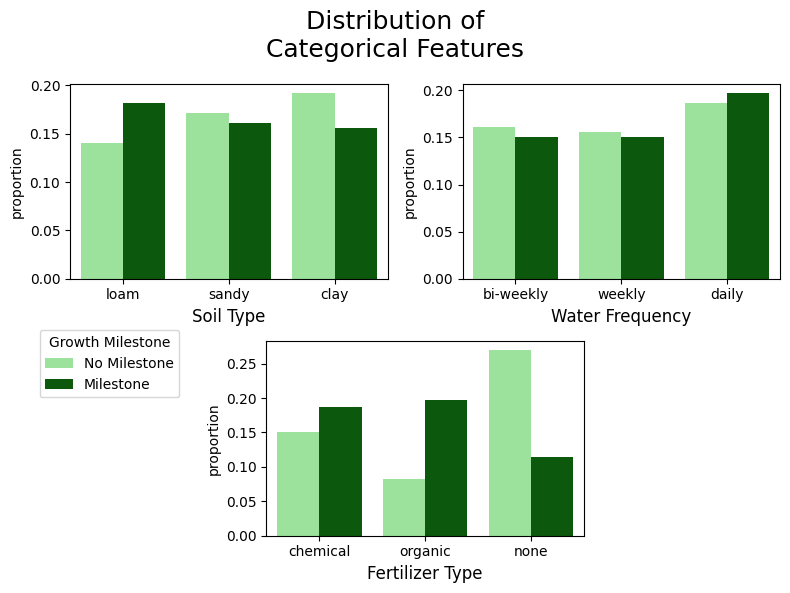
\includegraphics[width=0.95\textwidth]{./Resources/3_2.png}
                \caption{Distribución de los atributos Categóricos según el Crecimiento Significativo}
                \label{fig:dist_cat}
            \end{figure}

            Del gráfico, se puede destacar dos hechos. El atributo de \emph{Soil\_type} tiene un 
            impacto significativo en el crecimiento de las plantas, debido a que los suelos de tipo 
            franco (loam) afecta positivamente este fenómeno, mientras que un suelo de tipo arcilla 
            (clay) tiene el efecto negativo, esto es un indicio de una posible interacción fuerte que 
            repercute en el crecimiento significativo de una planta según el suelo en el que está plantada. 
            Mientras que al atributo \emph{Fertilizer\_Type} muestra un también	un impacto en el 
            crecimiento de las plantas, y este hecho es natural debido a que de aquí, la planta, obtiene 
            los diferentes nutrientes para su adecuado crecimiento, siendo así el como favorece 
            al crecimiento de una planta según el fertilizante que se use.
        }

    }
    \newpage

    \section{Metodología del Proyecto}\label{sec:meto}
    {
        \subsection{Preprocesamiento}
        {
            Del análisis realizado en la sección previa, en \ref{sec:eda} \nameref{sec:eda}, se 
            puede determinar que es necesario aplicar un adecuado preprocesamiento 
            de los atributos, así cómo también derivar otros que puedan crear otras 
            posibles interacciones. Por lo que se propone realizar lo siguiente:

            \begin{itemize}
                \item \textbf{Atributos Numéricos}: Los atributos que se generan los 
                que se obtienen después de aplicar las funciones $\sqrt{x}$, $\log_{10}{x}$, 
                $1/x$, $x^2$ y $x$ (denotando la función identidad), donde $x$ son los posibles 
                valores que pueden tomar los atributos numéricos. Después de generar los valores, 
                se la aplica la transformación de estandarización en cada uno de los atributos 
                derivados, esto se hace para que los valores estén en un rango de entre $-3$ y $3$ 
                o, equivalentemente, estén en unidades estándar.
                \item \textbf{Atributos Categóricos}: Debido a que los atributos pueden tomar 
                tres valores que no tienen una relación de orden plausible o clara, se tiene que 
                realizar una codificación haciendo uso de la codificación One-Hot, para obtener 
                una información más granular sobre las diferentes instancias. Después de esta 
                codificación no se le aplica ninguna otra transformación.
            \end{itemize}

            Debido a que el espacio de atributos creció a una dimensión relativamente grande, se 
            tiene que como parte del preprocesamiento se realiza una selección de atributos con 
            el fin de reducir el problema de la dimensionalidad y hacer que los modelos tengan un 
            mejor aprendizaje (capturen las relaciones importantes) mientras se reduce el coste 
            computacional tanto de entrenamiento como de predicción. Para ello: 

            \begin{itemize}
                \item \textbf{Atributos Numéricos}: Se selecciona los mejores $10$ atributos por 
                medio de Mutual Information (MI) \cite{sklearn_mutual_info}.
                \item \textbf{Atributos Categóricos}: Se seleccionan los mejores $6$ atributos por 
                medio del Estadístico $\chi^2$ \cite{sklearn_chi2}.
            \end{itemize}

            Ambas métricas permiten medir la misma noción de independencia respecto al target 
            (\emph{Growth\_Milestone}), es decir, se conversan o se usan los atributos que 
            son menos independientes del target con el fin de que el modelo pueda capturar 
            y aprender estas relaciones.\\

            Como parte del preprocesamiento, se incluye la separación del conjunto de datos original 
            en conjuntos de entrenamiento y de prueba, se hace uso del $25\%$ de las instancias como 
            instancias del conjunto de prueba.
        }
        
        \subsection{Modelos de Machine Learning}
        {
            Para realizar la tarea de clasificación del crecimiento de las plantas se hace uso, 
            principalmente, de modelos que permiten generar o propiciar bordes de decisión no 
            lineales, debido a que, por como se puede observar en \ref{sec:eda} \nameref{sec:eda}, 
            las clases del target no son linealmente separables, haciendo que los modelos que hacen 
            uso de bordes de decisión naive o lineales no puedan capturar adecuadamente los patrones 
            en los datos para clasificar una instancia de manera adecuada. Por ello, se hace uso de 
            los siguientes modelos e hiperparámetros a ajustar:\\

            \textbf{Support Vector Machine (SVM)}\\
            {
                El usar SVM permite añadir un capa adicional de interacción entre atributos debido a 
                que hace uso del truco del kernel que esto permite propiciar un mejor ambiente para 
                la separabilidad entre clases. Esto último hace que SVM sea un modelo predilecto para 
                tratar problemas de clasificación con clases sin separabilidad lineal, como lo es en 
                este caso. De los hiperparámetros que se encuentra en \cite{sklearn_svc}, se ajustan 
                los siguientes:
                \begin{itemize}
                    \item \emph{kernel}: Se escoge entre Poly (polinómico), RBF (Radial Basis 
                    Function) y Sigmoid.
                    \item \emph{C}: Parámetro de regularización. Se escogen valores reales en $[1e-10,5]$
                    \item \emph{gamma}: Coeficiente del kernel. Se escogen valores reales en $[0,2]$
                    \item \emph{degree}: Grado del polinomio. Ajustado únicamente en el kernel poly. Se escogen valores enteros en $[1,4]$ 
                    \item \emph{coef0}: Valor del coeficiente $x^0$. Ajustado únicamente en el kernel poly. Se escogen valores reales en $[0,2]$
                \end{itemize}
            }

            \textbf{Random Forest}\\
            {
                El usar Random Forest permite aprovechar de mejor manera las decisiones tomadas 
                por árboles de decisión simples, de profundidades bajas, gracias a que cuando 
                se combinan sus decisiones se reduce el sesgo y, por su entrenamiento, también 
                se reduce su varianza. Además de ello, al combinar varios árboles simples permite 
                el crear bordes de decisión más complejas, no lineales, beneficiándose así la 
                separabilidad entre clases. De los hiperparámetros que se encuentran en \cite{sklearn_forest}, 
                se ajustan los siguientes:
                \begin{itemize}
                    \item \emph{n\_estimators}: Cantidad de estimadores. Se escogen valores enteros en $[1,100]$ 
                    \item \emph{criterion}: Función para decidir que nodo aplicar el split. Se escoge entre gini y entropy
                    \item \emph{max\_depth}: Altura de máxima de los árboles de decisión. Se escogen valores enteros pequeños en $[1,3]$
                    \item \emph{min\_samples\_split}: Mínimo número de instancias en un nodo para aplicar la operación de split. Se escogen valores reales en $[1e-2,0.5]$
                \end{itemize}
            }

            \textbf{AdaBoost}\\
            {
                El usar árboles de decisión entrenados de forma secuencial para corregir los 
                errores generados por modelos previos mientras se mejora el poder predictivo, 
                permite generar bordes de decisión no lineales y más finos, es decir, que se 
                adecuen para generar una mayor separabilidad entre clases sin que se caiga en 
                un problema de varianza (esto justamente lo permite el ratio de aprendizaje). 
                De los hiperparámetros que se encuentran en \cite{sklearn_adaboost}, se ajustan 
                los siguientes:
                \begin{itemize}
                    \item \emph{estimator}: Estimador débil. Se hace uso de árboles de decisión con los parámetros defaults de \cite{sklearn_tree} y salvo \emph{max\_depth} que se escoge valores enteros en $[1,4]$
                    \item \emph{n\_estimators}: Cantidad de estimadores. Se escogen valores enteros en $[1,100]$ 
                    \item \emph{learning\_rate}: Peso que se aplica a cada modelo de manera secuencial. Se escogen valores reales en $[1e-3,2]$
                \end{itemize}
            }

            \textbf{Logistic Regression}\\
            {
                El decidir la clase de una instancia por medio de un borde decisión lineal podría 
                favorece en la comparativa contra modelos que generan bordes de decisión más complejos, 
                además de se explorar otra forma de generar interacciones por medio de combinaciones 
                lineales de atributos. Esto último permite que este modelo sea ampliamente usado 
                en problemas donde las clases están linealmente separadas. De los hiperparámetros 
                que se encuentran en \cite{sklearn_logistic}, se ajustan los siguientes:
                \begin{itemize}
                    \item \emph{C}: Parámetro de regularización. Se escogen valores reales en $[1e-10,5]$
                    \item \emph{penalty}: Tipo de penalización que se aplica a los parámetros. Se escoge entre $l1$ y $l2$
                    \item \emph{solver}: Algoritmo usado para optimizar los parámetros. Se escoge entre liblinear y saga (que admiten ambas penalizaciones)
                \end{itemize}
            }

            \textbf{K-Nearest Neighbors (KNN)}\\
            {
                El usar la distancia o similitud entre instancias permite determinar bordes de decisión	 
                no lineales entre las clases, debido a que usa operaciones no lineales para medir esta 
                noción de cercanía entre los diferentes puntos, permitiendo así la generación de la 
                separación entre clases. Esto último hace a KNN un modelo para modelar la predicción 
                de forma sencilla y con bajo coste computacional. De los hiperparámetros en \cite{sklearn_knn}, 
                se ajustan los siguientes:
                \begin{itemize}
                    \item \emph{n\_neighbors}: Cantidad de vecinos cercanos que se consideran. Se escogen valores enteros en $[3,50]$
                    \item \emph{weights}: La función de peso que se le aplica a cada vecino, importancia que tiene. Se escoge entre uniform y distance
                    \item \emph{p}: Potencia de métrica de Minkowski (por default, y solo se ajusta para esta métrica). Se escogen valores enteros en $[1,3]$
                    \item \emph{metric}: Métrica que se usa para medir distancia y similitud. Se escoge entre cosine y correlation
                \end{itemize}
            }
        }
    }
    \newpage

    \section{Experimentos y Discusión de Resultados}\label{sec:exp}
    {
        \subsection{Optimización de Hiperparámetros}
        {            
            Para realizar el fine-tunning de los hiperparámetros en cada uno de los modelos 
            propuestos en \ref{sec:meto} \nameref{sec:meto}, se hace uso Scikit Optimize, en 
            específico de BayesSearchCV \cite{skopt_bayes} para determinar los mejores hiperparámetros 
            por medio de métodos bayesianos (véase que funciona como Optuna \cite{optuna} pero 
            sin usar métodos sofisticados como algoritmos genéticos).
        }

        \subsection{Descripción de Experimentos}
        {
            Para el fine-tunning de hiperparámetros se hizo uso de la métrica \emph{accuracy}, debido 
            a que como las instancias del conjunto de datos se encuentran balanceadas \ref{sec:eda} \nameref{sec:eda} 
            y, bajo este escenario de balance, la métrica \emph{accuracy} se comporta como \emph{f1}, 
            y así permitiendo reducir el impacto de los falsos positivos (FP) y falsos negativos (FN) en 
            las predicciones, que esto se vuelve equivalentemente a reducir la sobrestimación y 
            subestimación, respectivamente, del crecimiento Significativo que una planta alcanza. 
            Y como BayesSearchCV \cite{skopt_bayes} se apoya en cross-validation, también se tiene 
            que definir la cantidad de pliegues o folds para realizar la validación de los hiperparámetros 
            candidatos a ser los mejores para un modelo, por ello se hace uso de $6$ pliegues debido a 
            que deja suficientes instancias para validar los hiperparámetros como de entrenamiento.   
        }

        \subsection{Evaluación de Resultados}
        {
            En base a los mejores modelos (hiperparámetros) encontrados por medio BayesSearchCV \cite{skopt_bayes}, 
            se evalúan tanto en el conjunto de entrenamiento como de prueba, se obtienen los siguientes 
            resultados tanto tabulados como gráficados:
            
            \begin{center}
                \begin{tabular}{lrrrrr}
                    \toprule
                        & SVM & Forest & AdaBoost & Logistic & KNN \\
                    \midrule
                        Accuracy & 0.638889 & 0.708333 & 0.694444 & 0.652778 & 1.000000 \\
                        Precision & 0.619565 & 0.666667 & 0.659574 & 0.657895 & 1.000000 \\
                        Recall & 0.770270 & 0.864865 & 0.837838 & 0.675676 & 1.000000 \\
                        F1 & 0.686747 & 0.752941 & 0.738095 & 0.666667 & 1.000000 \\
                    \bottomrule
                \end{tabular}
            \end{center}
            \begin{figure}[hbtp]
                \centering
                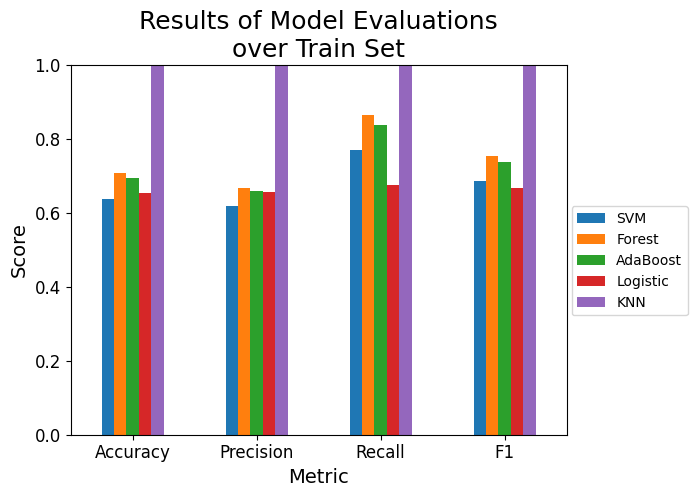
\includegraphics[width=0.9\textwidth]{./Resources/5_1.png}
                \caption{Puntajes de diferentes métricas de los Mejores Modelos en el Conjunto de Entrenamiento}
                \label{fig:res_train}
            \end{figure}

            \begin{figure}[hbtp]
                \centering
                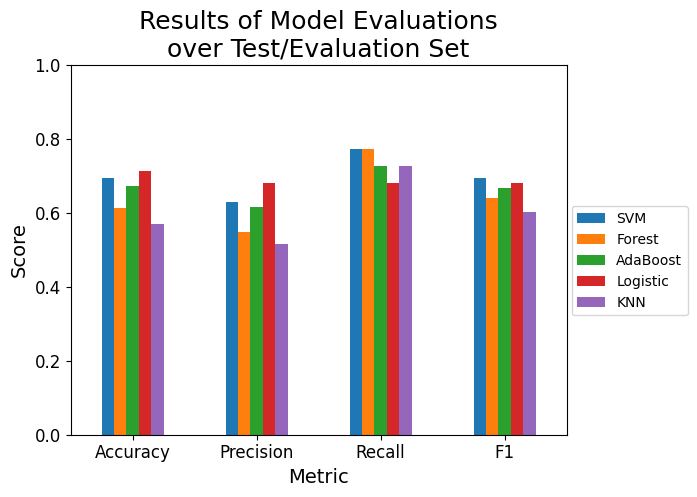
\includegraphics[width=0.9\textwidth]{./Resources/5_2.png}
                \caption{Puntajes de diferentes métricas de los Mejores Modelos en el Conjunto de Prueba}
                \label{fig:res_test}
            \end{figure}
            \begin{center}
                \begin{tabular}{lrrrrr}
                    \toprule
                        & SVM & Forest & AdaBoost & Logistic & KNN \\
                    \midrule
                        Accuracy & 0.693878 & 0.612245 & 0.673469 & 0.714286 & 0.571429 \\
                        Precision & 0.629630 & 0.548387 & 0.615385 & 0.681818 & 0.516129 \\
                        Recall & 0.772727 & 0.772727 & 0.727273 & 0.681818 & 0.727273 \\
                        F1 & 0.693878 & 0.641509 & 0.666667 & 0.681818 & 0.603774 \\
                    \bottomrule
                \end{tabular}
            \end{center}

            Haciendo de las principales métricas empleadas en clasificación se puede observar el 
            como se comportan los modelos en ambos conjuntos. Destacando como en Random Forest, 
            AdaBoost y KNN alcanzan puntajes más bajos en el conjunto de prueba que en el conjunto 
            de entrenamiento, destacando como KNN se encuentra sobreajustado de manera extrema. \\ 

            En cambio, en los modelos como SVM y Logistic Regression, tienen un mejor comportamiento 
            en el conjunto de prueba, haciendo que estos modelos sean lo más adecuados para el problema 
            presente. Debido a que ambos modelos emplean la separabilidad de clases como principio de 
            su funcionamiento, por lo que se tiene que los atributos generados en la etapa de preprocesamiento 
            fueron fructíferos para que el modelo sea capaz de aprender los patrones para poder distinguir 
            entre ambas clases del target.\\

            Para el caso de SVM, tiene un kernel polinómico de grado $1$ como sus mejores hiperparámetros; 
            y para el caso de Logistic Regression, su tipo de penalización es $l1$ es su mejor hiperparámetro. 
            Estas configuraciones muestran un indicio fuerte de que las clases son linealmente separables y, 
            de aquí, estos modelos obtengan los mejores resultados y que puedan ser robustos para la predicción 
            en nuevas instancias.
        }
    }
    \newpage

    \section{Análisis de Resultados}
    {
        En el marco de la agricultura industrial, una de las metas es alcanzar 
        la máxima producción y calidad (esto lleva consigo mayores ganancias), 
        por ello mientras más temprano se determinen las plantas que crecerán 
        de manera significativa va a permitir el focalizar los recursos en esas 
        plantas y, además, tomar medidas en las plantas que no tendrán un 
        crecimiento notorio. Por ello, se vuelve importante el construir modelos 
        que clasifiquen las plantas de manera adecuada bajo esta criteria, es decir, 
        incrementar los esfuerzos para que las plantas lleguen a tener un crecimiento 
        significativo o, equivalentemente, las condiciones para que logren esto.\\

        Lo anterior discutido se transforma, usando la jerga de Ciencia de Datos, reducir 
        los falsos positivos, es decir, indicar que una planta tendrá un crecimiento 
        notorio cuando en realidad no lo tendrá, esto último se puede ver como invertir 
        más tiempo y recursos en una planta que no propiciará un beneficio mayor que 
        las pérdidas generadas para su cuidado. De aquí se le tenga que dar más preferencia 
        a los modelos con un puntaje más alto en \emph{precision}, debido a que cuidan 
        el hecho de ``no mentir'' sobre el crecimiento de una planta, y esto se alinea con 
        el objetivo de maximizar la producción y calidad en las plantas.\\ 

        De la sección anterior, \ref{sec:exp} \nameref{sec:exp}, se puede determinar 
        que el mejor modelo para la tarea y el que mejor se ajusta es Logistic Regression, 
        esto lleva una implicación fuerte, y que está asociada a su definición, es que 
        los factores ambientales y de cuidado están en interacciones lineales simples, 
        por lo que se podría encontrar las combinaciones ideales para alcanzar la máxima 
        producción y calidad de forma sencilla y sin tanto coste computacional.\\

        Lo que pasa en los demás modelos, salvo con SVM, es que construyen relaciones 
        complejas entre los factores que impactan en el crecimiento de una planta, estas 
        relaciones se desvían mucho cuando se usan en otros casos, plantas, que no 
        pertenezcan a las usadas para el entrenamiento de los modelos, es decir, ver que 
        un patrón muy especifico y complejo se verifica en un conjunto de ejemplos como 
        que no siempre se sostiene en otros conjuntos de ejemplos, haciendo que les vaya 
        de peor manera al momento de determinar cuando una planta va a crecer notoriamente.
    }
    \newpage

    \section{Conclusiones}
    {}
    \newpage

    \printbibliography[heading=bibintoc,title={Referencias Bibliográficas}]

\end{document}